\newlecture[Chapter 4 - Inequalities][Sep 29, 2026]

\begin{theorem}[Markov's Inequality][4.1]
    If $X \geq 0$ a.s., then for all $a>0$, 
    \[P(X \geq a) \leq \frac{E(X)}{a}\]
    Proof: 
    \begin{quote}
        Define $Z(\omega) = a \cdot I\left\{X(\omega) \geq a\right\}$. Then, $Z\leq X$ a.s., and since $Z$ is simple,
        \[E(Z) = a\cdot P(X\geq a)\]
        \[P(X\geq a) = \frac{E(Z)}{a} \leq \frac{E(X)}{a}\]
    \end{quote}
\end{theorem}

\begin{theorem}[Chebyshev's Inequality][4.2]
    For all $t\geq 0$, 
    \[P(|X- E(X)|)\geq t \leq \frac{\Var(X)}{t^2}\]
    Proof: 
    \begin{quote}
        Apply Markov's inequality to $Y = [X-E(X)]^2$
        \\Both Chebyshev and Markov's inequality talk about
        \[P(X\geq \cdots) \quad \Leftarrow \quad \text{the tail probability}\]
            \begin{center}
                "Concentration of Probability Mass"
            \end{center}
        Where Markov uses the 1st moment, Chebyshev uses 2nd moment.
        \\What if we use other transformation/moments to quantify the tail probability?
        \\E.g. the exponential moment? $\Rightarrow$ Chernoff's Inequality
        \[M_X(t) = E[e^{tx}]\]
        \end{quote}
\end{theorem}

\begin{theorem}[Chernoff's Inequality][4.3]
    For all $t\geq 0$, \quad $P(X\geq E(X) + t) \leq \inf_{\lambda>0}M_X - E(X) (\lambda)e^{-\lambda t}$
    \[P(X\geq E(X) + t) \text{ roughly } P(\underbrace{X-E(X)}_{\substack{\text{distance between $X$} \\ \text{to its expected value}}}\geq t)\]
    \[\leq \inf_{\lambda>0} M_{X-E(X)} (\lambda)e^{-\lambda t}\]
    Proof:
    \begin{quote}
        the function $g(x) = e^x$ is monotonically increasing and non-negative.
        \[P(X-E(X) \geq t)\]
        \[=P(e^{E-E(X)} \geq e^t)\]
        \[=P(e^{\lambda(X-E(X))}\geq e^{\lambda t}) \quad \lambda \geq 0\]
        Since $e^{\lambda(X-E(X))} \geq 0$ a.s., we can apply Markov's inequality
        \[\leq \frac{E[e^\lambda (X - E(X))]}{e^{\lambda t}} \quad \text{where the num. is the }m_g f \quad M_{X-E(X)}\]
        We proved that 
        \[P(X-E(X) \geq t) \leq e^{-\lambda t} \cdot M_{X-E(X)}(\lambda)\]
        Since this inequality holds for any arbitrary $\lambda \geq 0$, we can take the inf:
        \[P(X-E(X) \geq t) \leq \inf_{\lambda>0}e^{-\lambda t}M_{X-E(X)}(\lambda)\]
    \end{quote}
\end{theorem}

\begin{theorem}[Hoeffding's Inequality][4.4]
    \begin{definition}[Convex Function][4.4.1]
        A function $f: \mathbb{R} \to \mathbb{R}$ is convex if for all $\lambda \in (0,1)$ and $x,y \in \mathbb{R}$
        \[f(\lambda x+(1-\lambda)y) \leq \lambda f(x)+ (1-\lambda)f(y)\]
        Any value between $x$ and $y$ can be represented as
        \[\lambda x+ (1-\lambda)y \text{ for } \lambda \in (0,1)\]
        \begin{center}
        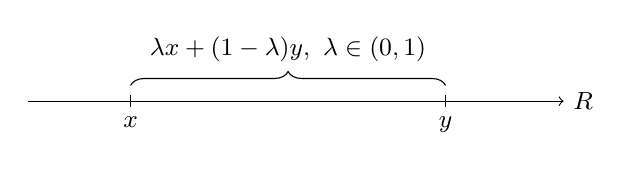
\begin{tikzpicture}[scale=1, every node/.style={font=\small}]
            \draw[->] (-0.3,0) -- (6.5,0) node[right]{$\mathbb{R}$};
            \draw (1,0.08) -- (1,-0.08) node[below]{$x$};
            \draw (5,0.08) -- (5,-0.08) node[below]{$y$};
            \draw[decorate, decoration={brace, amplitude=5pt}] (1,0.2) -- (5,0.2)
                node[midway, above=5pt]{\aside{$\lambda x + (1-\lambda)y,\ \lambda \in (0,1)$}};
        \end{tikzpicture}
        \end{center}
        if $\lambda \to 1$, then the value is closer to $x$. Vice versa for $\lambda \to 0$, the value is closer to $y$.
        \begin{center}
        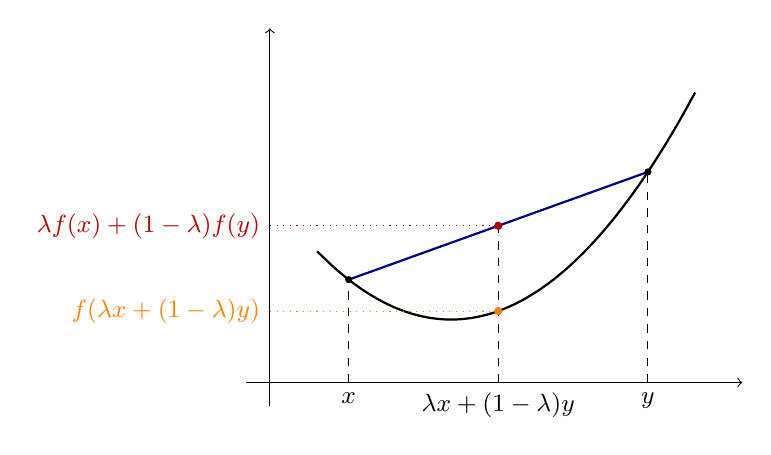
\begin{tikzpicture}[scale=1, every node/.style={font=\small}]
            \draw[->] (-0.3,0) -- (6,0);
            \draw[->] (0,-0.3) -- (0,4.5);
            \draw[thick, domain=0.6:5.4, smooth, variable=\x] plot ({\x}, {0.3*(\x-2.3)^2+0.8});
            % chord between x=1 and y=4.8
            \coordinate (A) at (1, {0.3*(1-2.3)^2+0.8});
            \coordinate (B) at (4.8, {0.3*(4.8-2.3)^2+0.8});
            \draw[thick, blue!55!black] (A) -- (B);
            \fill (A) circle (1.3pt); \fill (B) circle (1.3pt);
            % point lambda x + (1-lambda) y at x = 2.9 (lambda = 1/2)
            \coordinate (C) at (2.9, 1.991);
            \coordinate (F) at (2.9, {0.3*(2.9-2.3)^2+0.8});
            \draw[dashed] (1,0) -- (A);
            \draw[dashed] (4.8,0) -- (B);
            \draw[dashed] (2.9,0) -- (C);
            \draw[dotted, red!70!black] (0,0 |- C) -- (C);
            \draw[dotted, orange] (0,0 |- F) -- (F);
            \fill[red!70!black] (C) circle (1.5pt);
            \fill[orange] (F) circle (1.5pt);
            \node[below] at (1,0) {$x$};
            \node[below] at (2.9,0) {$\lambda x + (1-\lambda)y$};
            \node[below] at (4.8,0) {$y$};
            \node[anchor=east, red!70!black] at (0,0 |- C) {$\lambda f(x) + (1-\lambda)f(y)$};
            \node[anchor=east, orange] at (0,0 |- F) {$f(\lambda x + (1-\lambda)y)$};
        \end{tikzpicture}
        \end{center}
        Convexity: $f(\lambda x+ (1-\lambda)y) \leq \lambda f(x) + (1-\lambda)f(y)$
        \\ \aside{$\Rightarrow$ the function is under the straight line}
    \end{definition}
    \begin{lemma}[Hoeffding's Lemma][4.4.2]
        If $Y$ satisfies $E(Y) = 0$ and $a\leq Y \leq b$ a.s., then for all $\lambda > 0$
        \[M_Y(\lambda) \leq e^{\lambda^2(b-a)^2/8}\]
        Proof:
        \begin{quote}
            Since $a \leq Y \leq b$ a.s., $Y = \alpha \cdot a + (1-\alpha)\cdot b$.
            \\ Transforming $Y \Rightarrow \alpha$, where $0 \leq \alpha \leq 1$,
            \[\alpha = \frac{b-Y}{b-a}, \qquad 1-\alpha = \frac{Y-a}{b-a}\]
            Also, since the function $e^{\lambda y}$ is convex,
            \[e^{\lambda(\alpha a + (1-\alpha)b)} \leq \alpha e^{\lambda a} + (1-\alpha)e^{\lambda b}\]
            Apply $f(y) = e^{\lambda y}$ transformation to r.v.\ $Y$:
            \[e^{\lambda Y} \leq \alpha e^{\lambda a} + (1-\alpha)e^{\lambda b} = \frac{b-Y}{b-a}e^{\lambda a} + \frac{Y-a}{b-a}e^{\lambda b}\]
            Take expectation on both sides:
            \[E[e^{\lambda Y}] \leq E\Big[\frac{b-\overbrace{Y}^{\aside{random var.}}}{b-a}\underbrace{e^{\lambda a}}_{\aside{constant}}\Big] + E\Big[\frac{Y-a}{b-a}\underbrace{e^{\lambda b}}_{\aside{constant}}\Big]\]
            \[= \frac{b-E(Y)}{b-a}e^{\lambda a} + \frac{E(Y)-a}{b-a}e^{\lambda b}\]
            \[= \underbrace{\frac{b}{b-a}}_{p}e^{\lambda a} + \frac{-a}{b-a}e^{\lambda b} \qquad (\text{since } E(Y) = 0)\]
            Next, we let $p = \frac{b}{b-a}$:
            \[E[e^{\lambda Y}] = pe^{\lambda a} + (1-p)e^{\lambda b}\]
            We take log on RHS:
            \[\log\{E[e^{\lambda Y}]\} \leq \log\{pe^{\lambda a} + (1-p)e^{\lambda b}\}\]
            \[= \log\{e^{\lambda a}[p + (1-p)e^{\lambda(b-a)}]\}\]
            \[= \underbrace{\lambda a}_{\textcolor{blue!55!black}{=(p-1)u}} + \log[p + (1-p)e^{\lambda(b-a)}]\]
            \[\textcolor{blue!55!black}{(p-1)u = \left(\frac{b}{b-a}-1\right)(b-a)\lambda = \frac{a}{b-a}(b-a)\lambda = a\lambda}\]
            Next, let $u = (b-a)\lambda$:
            \[= (p-1)u + \log[p + (1-p)e^u] = \varphi(u)\]
            \[\varphi(0) = 0, \qquad \varphi'(u) = (p-1) + \frac{(1-p)e^u}{p+(1-p)e^u}, \qquad \varphi'(0) = 0\]
            \[\varphi(u) = \underbrace{\varphi(0)}_{0} + \underbrace{\varphi'(0)}_{0}u + \frac{\varphi''(\xi)}{2}u^2 + \cdots \qquad \text{(Taylor's Expansion at } u = 0)\]
            For some $\xi$ between $0$ and $u$, \quad $\varphi(u) = \frac{1}{2}\varphi''(\xi)u^2$
            \[\varphi''(u) = \frac{p(1-p)e^u}{[p+(1-p)e^u]^2} \leq \frac{1}{4}\]
            \[\Rightarrow \varphi(u) \leq \frac{1}{8}u^2\]
            \[\Rightarrow \log\{E[e^{\lambda Y}]\} \leq \frac{1}{8}u^2 = \frac{(b-a)^2\lambda^2}{8} \quad \text{as } u = (b-a)\lambda\]
            \[\Rightarrow M_Y(\lambda) \leq e^{\frac{(b-a)^2\lambda^2}{8}}\]
            \hfill $\square$
        \end{quote}
    \end{lemma}
    \heading{Hoeffding's Inequality:}
    Suppose $X_1, X_2, \dots, X_n, \dots$ are indep.\ with $a_i \leq X_i \leq b_i$ for all $i$.
    \\ Then letting $S_n = \sum_{i=1}^n X_i$, for all $t > 0$,
    \[P(|S_n - E(S_n)| \geq t) \leq 2 \cdot e^{-\frac{2t^2}{\sum_{i=1}^n (b_i - a_i)^2}}\]
    Proof:
    \begin{quote}
        We first prove the $P(S_n - E(S_n) \geq t)$ part.
        \\ Applying Chernoff's inequality,
        \[P(S_n - E(S_n) \geq t) \leq e^{-\lambda t}E[e^{\lambda(S_n - E(S_n))}]\]
        \[S_n - E(S_n) = \sum_{i=1}^n (X_i - E(X_i)), \qquad S_n = \sum_{i=1}^n X_i\]
        \[e^{\lambda(S_n - E(S_n))} = e^{\lambda\sum_{i=1}^n (X_i - E(X_i))} = \prod_{i=1}^n \underbrace{e^{\lambda[X_i - E(X_i)]}}_{\textcolor{blue!55!black}{M_{X_i - E(X_i)}(\lambda)}}\]
        \[M_{S_n - E(S_n)}(\lambda) = \prod_{i=1}^n M_{X_i - E(X_i)}(\lambda)\]
        Applying Hoeffding's Lemma: \quad $M_{X_i - E(X_i)}(\lambda) \leq e^{\frac{(b_i - a_i)^2\lambda^2}{8}}$
        \[M_{S_n - E(S_n)}(\lambda) \leq \prod_{i=1}^n e^{\frac{(b_i-a_i)^2\lambda^2}{8}} = e^{\frac{\lambda^2}{8}\sum_{i=1}^n (b_i - a_i)^2}\]
        Combine with Chernoff's inequality:
        \[P(S_n - E(S_n) \geq t) \leq e^{-\lambda t + \frac{\lambda^2}{8}\sum_{i=1}^n (b_i - a_i)^2}\]
        Rearrange, we have Hoeffding's inequality.
        \hfill $\square$
    \end{quote}
\end{theorem}
